\documentclass[conference, a4paper]{IEEEtran}

\usepackage[english]{babel}
\usepackage{booktabs}
\usepackage{amsmath}
\usepackage{graphicx}
\usepackage{algorithm}
\usepackage{algpseudocode}
\usepackage{tabularx}
\usepackage{array}
\usepackage{cite}
\usepackage{hyperref}

\begin{document}

\title{HoneyMed: A Protocol-Aware Honeypot Framework for Real-Time Threat Classification in Internet of Medical Things Networks}

\author{
\IEEEauthorblockN{1\textsuperscript{st} Author Names}
\IEEEauthorblockA{\textit{Department of Computer Science} \\
\textit{Name of University/College}\\
City, Country \\
author1@example.edu}
\and
\IEEEauthorblockN{2\textsuperscript{nd} Author Name}
\IEEEauthorblockA{\textit{Department of Computer Science} \\
\textit{Name of University/College}\\
City, Country \\
author2@example.edu}
}

\maketitle

\begin{abstract}
Internet of Medical Things (IoMT) deployments connect bedside monitors, hospital messaging systems, imaging infrastructure, and remote-care devices. This connectivity improves clinical visibility, but it also exposes legacy protocols, weak credentials, and lightly monitored interfaces to reconnaissance, denial-of-service, brute-force, and protocol-specific attacks. This paper presents HoneyMed, a protocol-aware honeypot framework that emulates selected healthcare and IoT services, captures suspicious interactions, converts them into machine-learning features, classifies attack behavior in near real time, and stores SHA-256 hashes for ledger-ready evidence handling. The implementation includes a VitalSync Pro 3000 patient-monitor decoy, HL7, DICOM, MQTT, and SSH-facing services, a feature extraction pipeline, Random Forest, Decision Tree, and XGBoost classifiers, a REST API, a Streamlit security dashboard, and simulated SIEM response hooks. A fresh controlled experiment on a 5,000-sample HoneyMed dataset shows that Random Forest achieved 98.50\% accuracy and a 98.49\% weighted F1-score, with the strongest feature contributions coming from payload entropy, payload size, credential indicators, and scan-like behavior. The running prototype captured attack-simulation traffic and rendered live dashboards with classified events and blockchain-ready hashes. These results show that combining deception, explainable tabular features, and lightweight classifiers can provide practical threat visibility for IoMT security testbeds without touching production medical assets.
\end{abstract}

\begin{IEEEkeywords}
Internet of Medical Things, honeypot, intrusion detection, cyber deception, machine learning, healthcare cybersecurity
\end{IEEEkeywords}

\section{Introduction}
The Internet of Medical Things (IoMT) is becoming a normal part of modern healthcare infrastructure. Patient monitors, infusion-related controllers, imaging workflows, telemetry gateways, and remote-care devices exchange data across hospital networks and cloud-connected services. The same connectivity that enables faster monitoring and decision support also increases exposure. Many clinical environments still contain long-lived devices, limited patch windows, shared administrative workflows, and communication protocols that were designed for trusted hospital networks rather than hostile networks.

The operational risk is different from ordinary enterprise information technology. A successful attack against a medical device ecosystem may affect confidentiality, but it may also interrupt monitoring, delay diagnosis, mislead clinical staff, or create unsafe operating conditions. Recent IoMT security work has therefore emphasized not only high detection accuracy, but also low-latency response, explainability, and privacy-preserving collaboration across institutions \cite{lipsa2025interpretable,hosain2025xaixgboost,tawfik2025fedmedsecure}. Even so, many proposed systems remain dataset-centered: they classify benchmark records, but do not show how suspicious protocol interactions are captured, normalized, displayed, and prepared for incident response in an operational workflow.

Honeypots provide a complementary signal. A production patient monitor should receive legitimate clinical traffic, but a decoy patient monitor placed in a monitored network segment should not be contacted by normal users. Any interaction with the decoy is therefore valuable telemetry. A healthcare honeypot can expose believable web, HL7, DICOM, MQTT, and embedded-device surfaces, capture probing behavior safely, and route those observations into a detection pipeline.

HoneyMed addresses this practical gap. The system combines medical-protocol deception, structured feature extraction, machine-learning classification, dashboard visualization, and ledger-ready hashing. The contribution is not a new classifier alone; rather, it is an end-to-end IoMT security prototype that shows how decoys, supervised models, and response interfaces can work together.

The main contributions of this paper are:
\begin{itemize}
    \item A multi-service IoMT honeypot architecture that emulates a patient-monitor web interface and protocol listeners for HL7, DICOM, MQTT, and SSH-like embedded-device access.
    \item A feature extraction and evidence pipeline that converts raw sessions into tabular ML features while computing SHA-256 hashes for audit and future blockchain submission.
    \item A current experimental evaluation of Random Forest, Decision Tree, and XGBoost classifiers on a 5,000-sample HoneyMed dataset, with accuracy, F1-score, confusion-matrix, and feature-importance analysis.
    \item A working dashboard and REST API that display live classified events, attack distributions, targeted services, and blockchain-ready hashes from a running attack simulation.
\end{itemize}

\section{Related Work and Literature Survey}

\subsection{IoMT Intrusion Detection}
Recent IoMT intrusion-detection research has moved toward high-accuracy models that also expose the reasons behind a prediction. Lipsa et al. proposed an interpretable dimensional reduction approach for IoMT attack detection and reported that a Random Forest explainable model reached 99\% accuracy on CICIoMT2024, outperforming XGBoost, Decision Tree, and SVM baselines in their study \cite{lipsa2025interpretable}. Hosain and Cakmak introduced XAI-XGBoost, combining sampling, recursive feature elimination, optimized XGBoost, SHAP, and LIME; their framework achieved 99.22\% accuracy on WUSTL-EHMS-2020 while emphasizing that interpretability is essential in healthcare security \cite{hosain2025xaixgboost}. Ramya et al. proposed AIDT, a probabilistic neural network and particle-swarm feature-extraction technique for secure IoMT communication, reporting 96.4\% accuracy \cite{ramya2025aidt}.

Other 2026 work extends the classifier space. Abdelhaq et al. proposed a hybrid XGBoost--SVM ensemble for IoMT cyberattack detection and reported 98.04\% accuracy on WUSTL-EHMS-2020 with validation against TON-IoT and CICIDS2017 \cite{abdelhaq2026hybrid}. Jaiswal et al. proposed a Tsetlin Machine-driven IDS for next-generation IoMT security, reporting 99.5\% binary accuracy and 90.7\% multiclass accuracy on CICIoMT2024 \cite{jaiswal2026tsetlin}. These studies validate the importance of tabular and interpretable learning for IoMT traffic. HoneyMed follows this direction by using transparent, low-cost features and tree-based classifiers, but it ties the classifier to an actual deception and event-ingestion pipeline.

\subsection{Federated, Blockchain, and Privacy-Preserving Directions}
Privacy-preserving collaboration is another major theme. Hassan et al. surveyed IoMT intrusion detection and organized recent work around datasets, deployment strategies, response mechanisms, federated learning, blockchain validation, and explainable AI \cite{hassan2025survey}. FedMedSecure combines federated few-shot learning, cross-attention, explainable AI, and differential privacy for collaborative healthcare cybersecurity, reporting strong results on CICIoMT2024 and cross-dataset evaluation while reducing communication overhead \cite{tawfik2025fedmedsecure}. Durga et al. proposed a federated TinyGAN framework for lightweight IoMT malware detection, reporting 99.52\% F1-score after 20 federated training rounds \cite{durga2026tinygan}.

HoneyMed does not implement full federated learning, but its design prepares the local system for collaborative extensions. Raw sessions remain local, while classified summaries and SHA-256 hashes can be exported through an API or submitted to a ledger. This design matches the direction identified in recent survey work: hospitals need ways to share indicators and trust signals without exposing protected health information or raw network payloads \cite{hassan2025survey}.

\subsection{Edge Architectures and Cyber Deception}
IoMT detection also depends on where computation happens. Islam et al. proposed a hybrid fog-edge architecture for real-time IoMT monitoring and reported latency, energy, bandwidth, and threat-detection improvements compared with cloud-only processing \cite{islam2025fogedge}. HoneyMed uses a similar operational intuition: capture and first-stage classification should be close to the decoy services so that suspicious behavior is visible quickly.

Cyber deception research provides the second foundation. Guan et al. presented HoneyIoT, a learning-based IoT honeypot that uses reinforcement learning to adaptively engage attackers \cite{guan2025honeyiot}. Li et al. proposed a reinforcement-learning strategy for deploying multiple deception resources and reported improved defensive success probability and deployment cost trade-offs \cite{li2025deception}. Sladic et al. introduced VelLMes, a high-interaction AI deception framework that can simulate multiple services and was evaluated with human attackers and Internet-deployed honeypots \cite{sladic2025vellmes}. These works show that deception is moving beyond static banners toward adaptive, realistic engagement. HoneyMed is narrower than those systems because it focuses on a medical testbed, but it contributes a domain-specific decoy stack connected to ML classification and healthcare-oriented evidence handling.

\subsection{Gap Analysis}
The literature shows three useful but often separate streams: accurate IoMT classifiers, privacy-preserving collaborative learning, and deception-based capture. The practical gap is their integration. A hospital security team needs a system that can safely receive attacker traffic, extract medically meaningful protocol context, classify activity with low operational cost, and display evidence in a form suitable for response. HoneyMed is designed around that integration rather than around a single model score.

\section{Proposed Methodology}

\subsection{System Architecture}
HoneyMed uses four cooperating zones: a clinical decoy zone, an evidence pipeline, a detection core, and an operations zone. Fig. \ref{fig:architecture} shows the architecture and data flow. The decoy zone exposes believable attack surfaces. The evidence pipeline normalizes sessions, extracts features, computes hashes, and stores classified windows. The detection core loads trained models and scores events. The operations zone serves dashboard views, API responses, hash feeds, and simulated SIEM actions.

\begin{figure*}[!t]
  \centering
  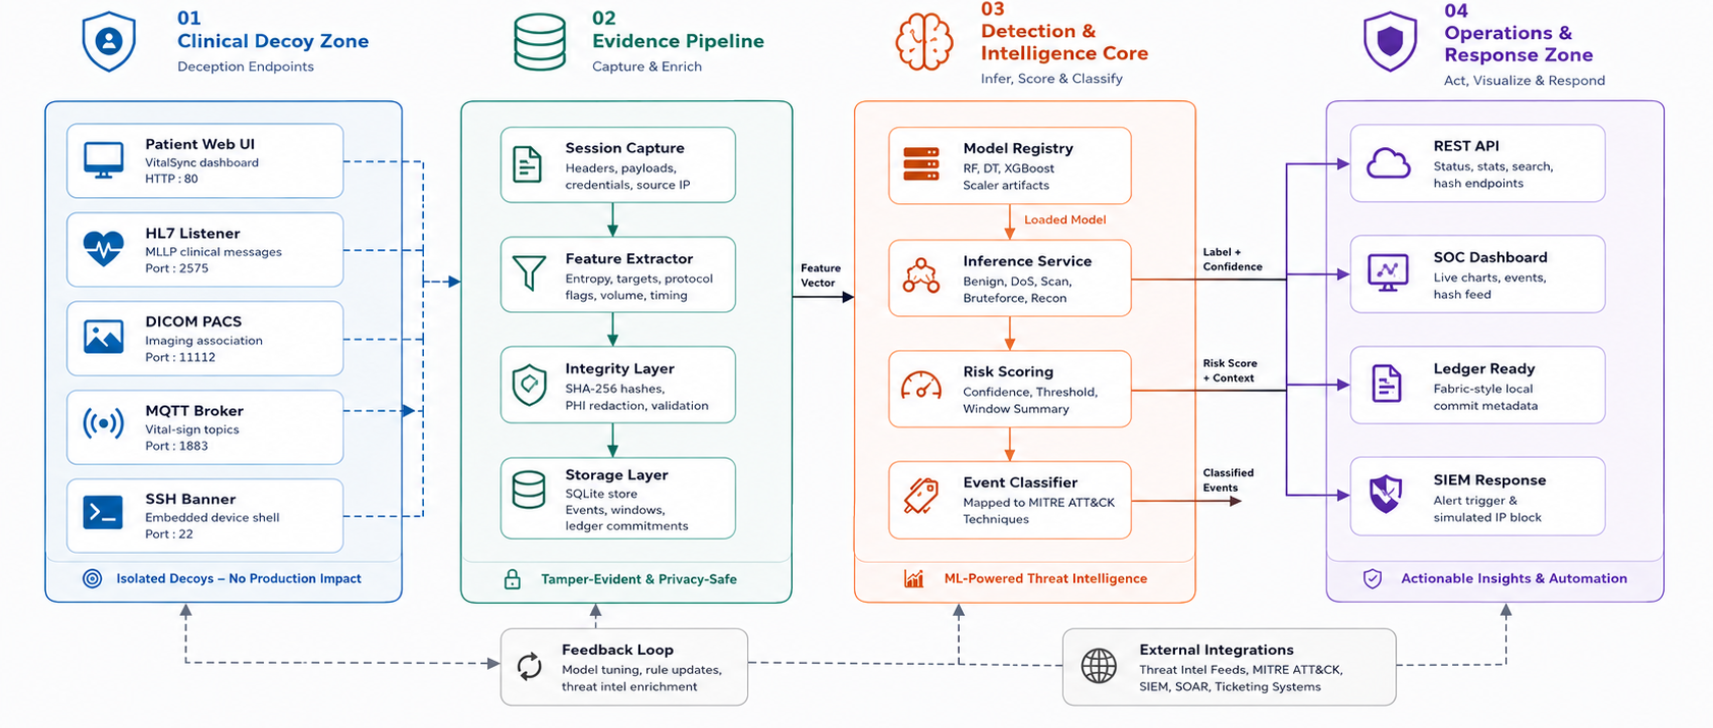
\includegraphics[width=\textwidth]{artifacts/figures/fig04_system_architecture.png}
  \caption{HoneyMed system architecture showing decoy services, evidence processing, ML inference, dashboard/API outputs, ledger-ready hashes, and SIEM response hooks.}
  \label{fig:architecture}
\end{figure*}

The edge emulation layer exposes five services: a web patient-monitor interface on port 80, an HL7 MLLP listener on port 2575, a DICOM PACS listener on port 11112, an MQTT broker-style telemetry surface on port 1883, and an SSH-like embedded-device banner on port 22. The web interface emulates a fictitious VitalSync Pro 3000 device. Fig. \ref{fig:vitalsync-decoy} shows the running patient-monitor dashboard captured during the project execution.

\begin{figure}[!t]
  \centering
  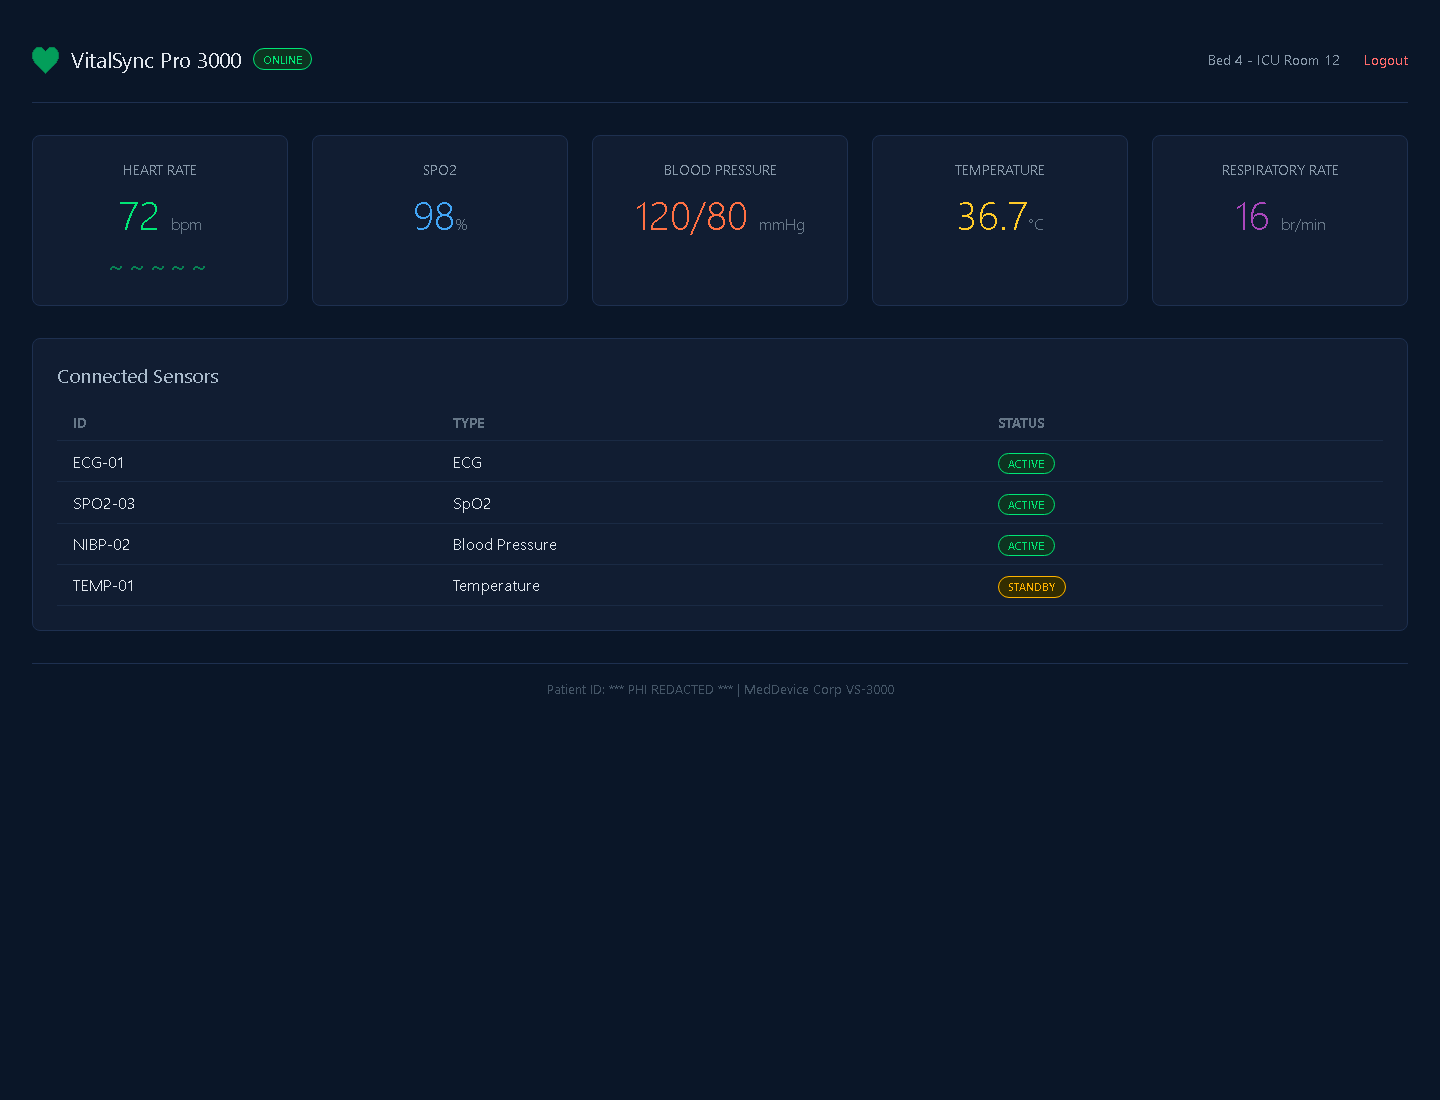
\includegraphics[width=\linewidth]{artifacts/screenshots/fig01_vitalsync_patient_monitor.png}
  \caption{VitalSync Pro 3000 decoy patient-monitor dashboard served by the running Layer 1 web honeypot.}
  \label{fig:vitalsync-decoy}
\end{figure}

\subsection{Event Flow}
When a client interacts with a decoy endpoint, HoneyMed records the timestamp, source address, source port, service name, event type, request metadata, and payload summary. The feature extractor then computes fields such as time-of-day indicators, target port, payload size, payload entropy, protocol flags, credential presence, scan-like behavior, request count, and status code. These values form the model input vector.

The classifier assigns one of five labels: Benign, DoS, PortScan, BruteForce, or Reconnaissance. Each event also receives a confidence score. When the event is malicious, the response layer can generate an alert or simulated IP block. In parallel, the integrity layer computes a SHA-256 digest that can be stored locally or sent to a future Hyperledger Fabric ledger. The current prototype runs in local ledger mode.

\subsection{Algorithmic Summary}
Algorithms \ref{alg:listener}--\ref{alg:predict} summarize the implementation logic. The listener records protocol interactions, the pipeline converts new events into features, and the predictor returns the class and confidence score.

\begin{algorithm}[!t]
\caption{Honeypot listener service}\label{alg:listener}
\begin{algorithmic}[1]
\Require $port, protocol$
\State $sock \gets \text{CreateSocket(TCP/IP)}$
\State $sock.\text{Bind}(0.0.0.0, port)$
\State $sock.\text{Listen}()$
\While{service is running}
    \State $client, addr \gets sock.\text{Accept}()$
    \State $\text{SendDecoyBanner}(client, protocol)$
    \State $payload \gets client.\text{ReceiveData}()$
    \State $event \gets \{time, addr, protocol, payload\}$
    \State $\text{AppendStructuredLog}(event)$
    \State $client.\text{Close}()$
\EndWhile
\end{algorithmic}
\end{algorithm}

\begin{algorithm}[!t]
\caption{Real-time evidence pipeline}\label{alg:pipeline}
\begin{algorithmic}[1]
\While{pipeline is running}
    \State $events \gets \text{ReadCapturedEvents}()$
    \ForAll{$event \in events$}
        \State $x \gets \text{ExtractFeatures}(event)$
        \State $digest \gets \text{SHA256}(event)$
        \State $label, conf \gets \text{Predict}(x)$
        \State $\text{Store}(event, x, label, conf, digest)$
        \If{$label \neq \text{Benign}$}
            \State $\text{TriggerResponse}(event.ip, label, conf)$
        \EndIf
    \EndFor
    \State $\text{Sleep}(5\text{s})$
\EndWhile
\end{algorithmic}
\end{algorithm}

\begin{algorithm}[!t]
\caption{ML inference predictor}\label{alg:predict}
\begin{algorithmic}[1]
\Require $feature\_vector$
\Ensure $class, confidence$
\State $model \gets \text{Load}(\text{attack\_classifier.pkl})$
\State $scaler \gets \text{Load}(\text{feature\_scaler.pkl})$
\State $z \gets scaler.\text{Transform}(feature\_vector)$
\State $class \gets model.\text{Predict}(z)$
\State $probs \gets model.\text{PredictProba}(z)$
\State \Return $class, \max(probs)$
\end{algorithmic}
\end{algorithm}

\section{Experimental Setup}

\subsection{Training Dataset and Models}
The current evaluation uses a freshly generated HoneyMed synthetic dataset with 5,000 labeled samples. The class distribution was 2,000 Benign samples and 750 samples each for DoS, PortScan, BruteForce, and Reconnaissance. The data were split using an 80/20 stratified train-test split, producing 4,000 training samples and 1,000 held-out test samples. The evaluated models were Random Forest, Decision Tree, and XGBoost. The metrics were accuracy, weighted precision, weighted recall, weighted F1-score, five-fold cross-validated weighted F1-score, and training time.

\subsection{Runtime Testbed}
The project was executed locally with the full HoneyMed stack: honeypot services, real-time pipeline, dashboard API, and Streamlit dashboard. The attack simulator then generated port scanning, web login brute-force attempts, API enumeration, HTTP flood traffic, HL7 injection messages, MQTT probes, and a DICOM association probe against localhost. The simulator saved a fresh attack log with 94 high-level events, while the live pipeline expanded HTTP flood traffic into a larger event stream and displayed the results in the dashboard.

\section{Results and Analysis}

\subsection{Model Performance}
Table \ref{tab:ml_perf} gives the current training results. Random Forest achieved the strongest held-out test performance, with 98.50\% accuracy and 98.49\% weighted F1-score. Decision Tree was close behind, while XGBoost was slightly lower on this generated dataset. Fig. \ref{fig:model-metrics} visualizes the same comparison.

\begin{table}[!t]
\centering
\caption{Current HoneyMed classifier results on 5,000 generated samples}
\label{tab:ml_perf}
\begin{tabular}{@{}lccccc@{}}
\toprule
\textbf{Model} & \textbf{Acc.} & \textbf{Prec.} & \textbf{Rec.} & \textbf{F1} & \textbf{CV F1} \\ \midrule
Random Forest & \textbf{98.50} & \textbf{98.53} & \textbf{98.50} & \textbf{98.49} & \textbf{99.02} \\
Decision Tree & 98.40 & 98.43 & 98.40 & 98.39 & 98.45 \\
XGBoost & 98.30 & 98.32 & 98.30 & 98.29 & 98.80 \\ \bottomrule
\end{tabular}
\end{table}

\begin{figure}[!t]
  \centering
  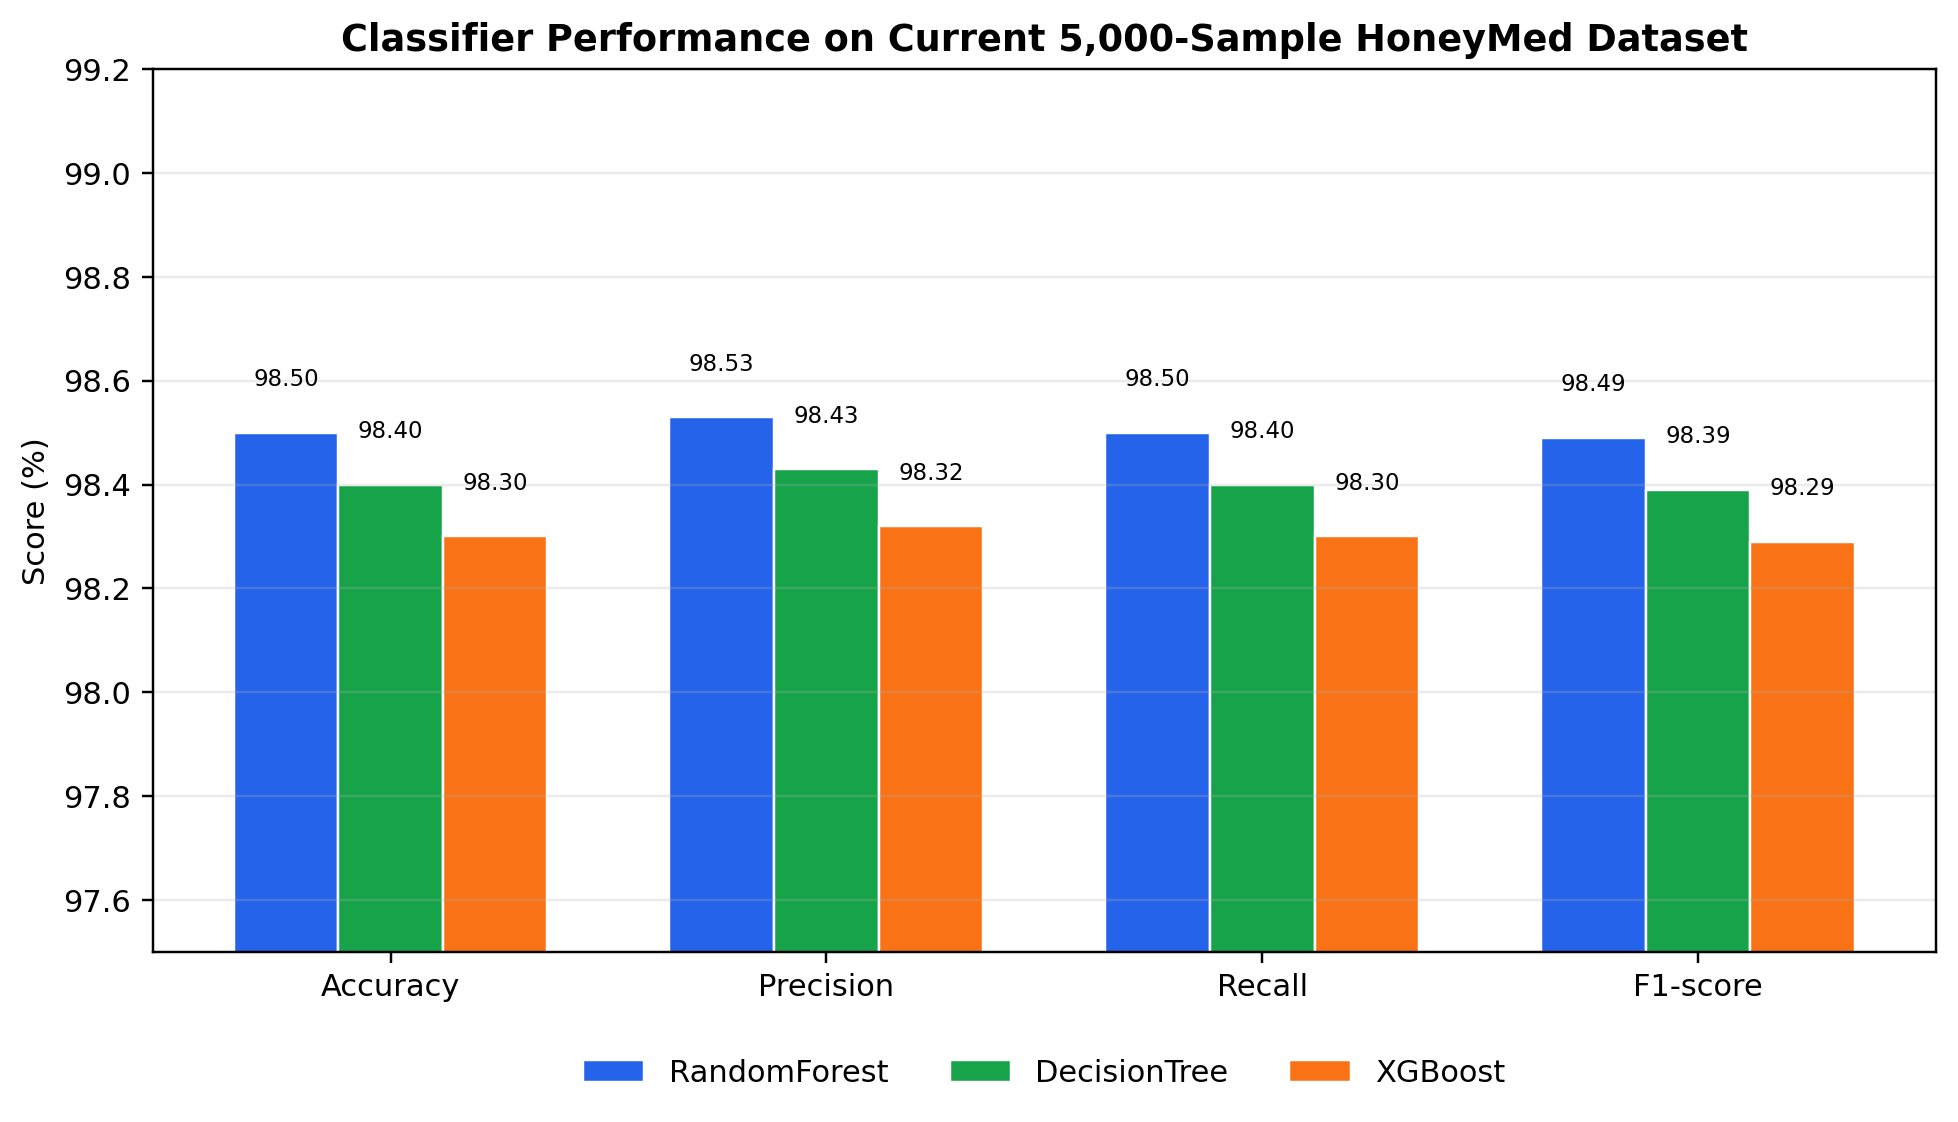
\includegraphics[width=\linewidth]{artifacts/figures/fig05_model_metrics.png}
  \caption{Accuracy, precision, recall, and F1-score for the three trained classifiers.}
  \label{fig:model-metrics}
\end{figure}

The confusion matrix in Fig. \ref{fig:confusion} shows that DoS and PortScan were classified perfectly in the held-out test set. BruteForce had one false Benign prediction. Reconnaissance was the hardest class, with 12 of 150 samples predicted as Benign. This error pattern is plausible because some reconnaissance behavior can resemble low-volume normal probing unless protocol context, scan flags, and payload structure are strong enough.

\begin{figure}[!t]
  \centering
  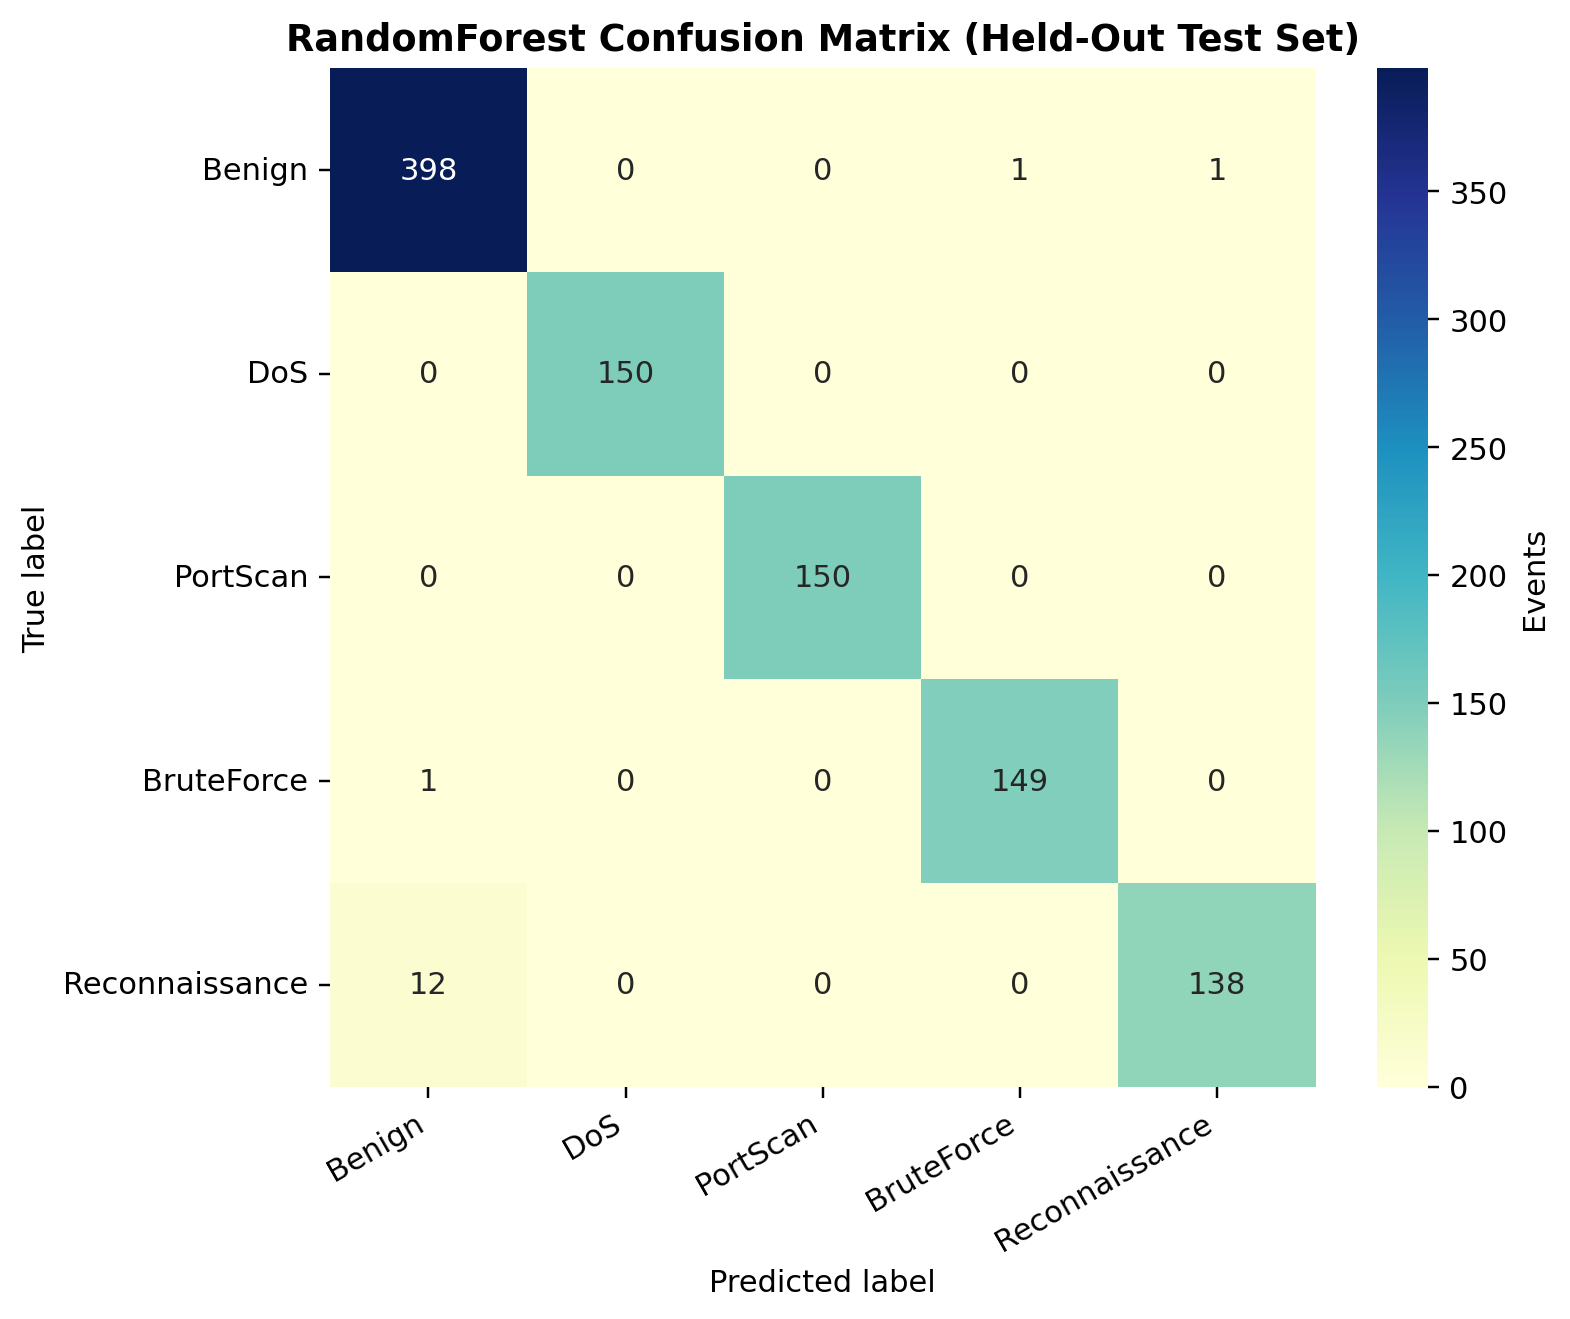
\includegraphics[width=\linewidth]{artifacts/figures/fig06_confusion_matrix.png}
  \caption{Random Forest confusion matrix on the held-out test split.}
  \label{fig:confusion}
\end{figure}

Fig. \ref{fig:importance} reports the top Random Forest feature contributions. Payload entropy and payload size dominated the model, followed by credential indicators, scan-like behavior, status code, target port, high-volume traffic, request count, and protocol flags. These features align with the attack simulator: brute-force behavior creates credential artifacts, DoS traffic creates volume signals, and reconnaissance or scans affect target-port and scan-like fields.

\begin{figure}[!t]
  \centering
  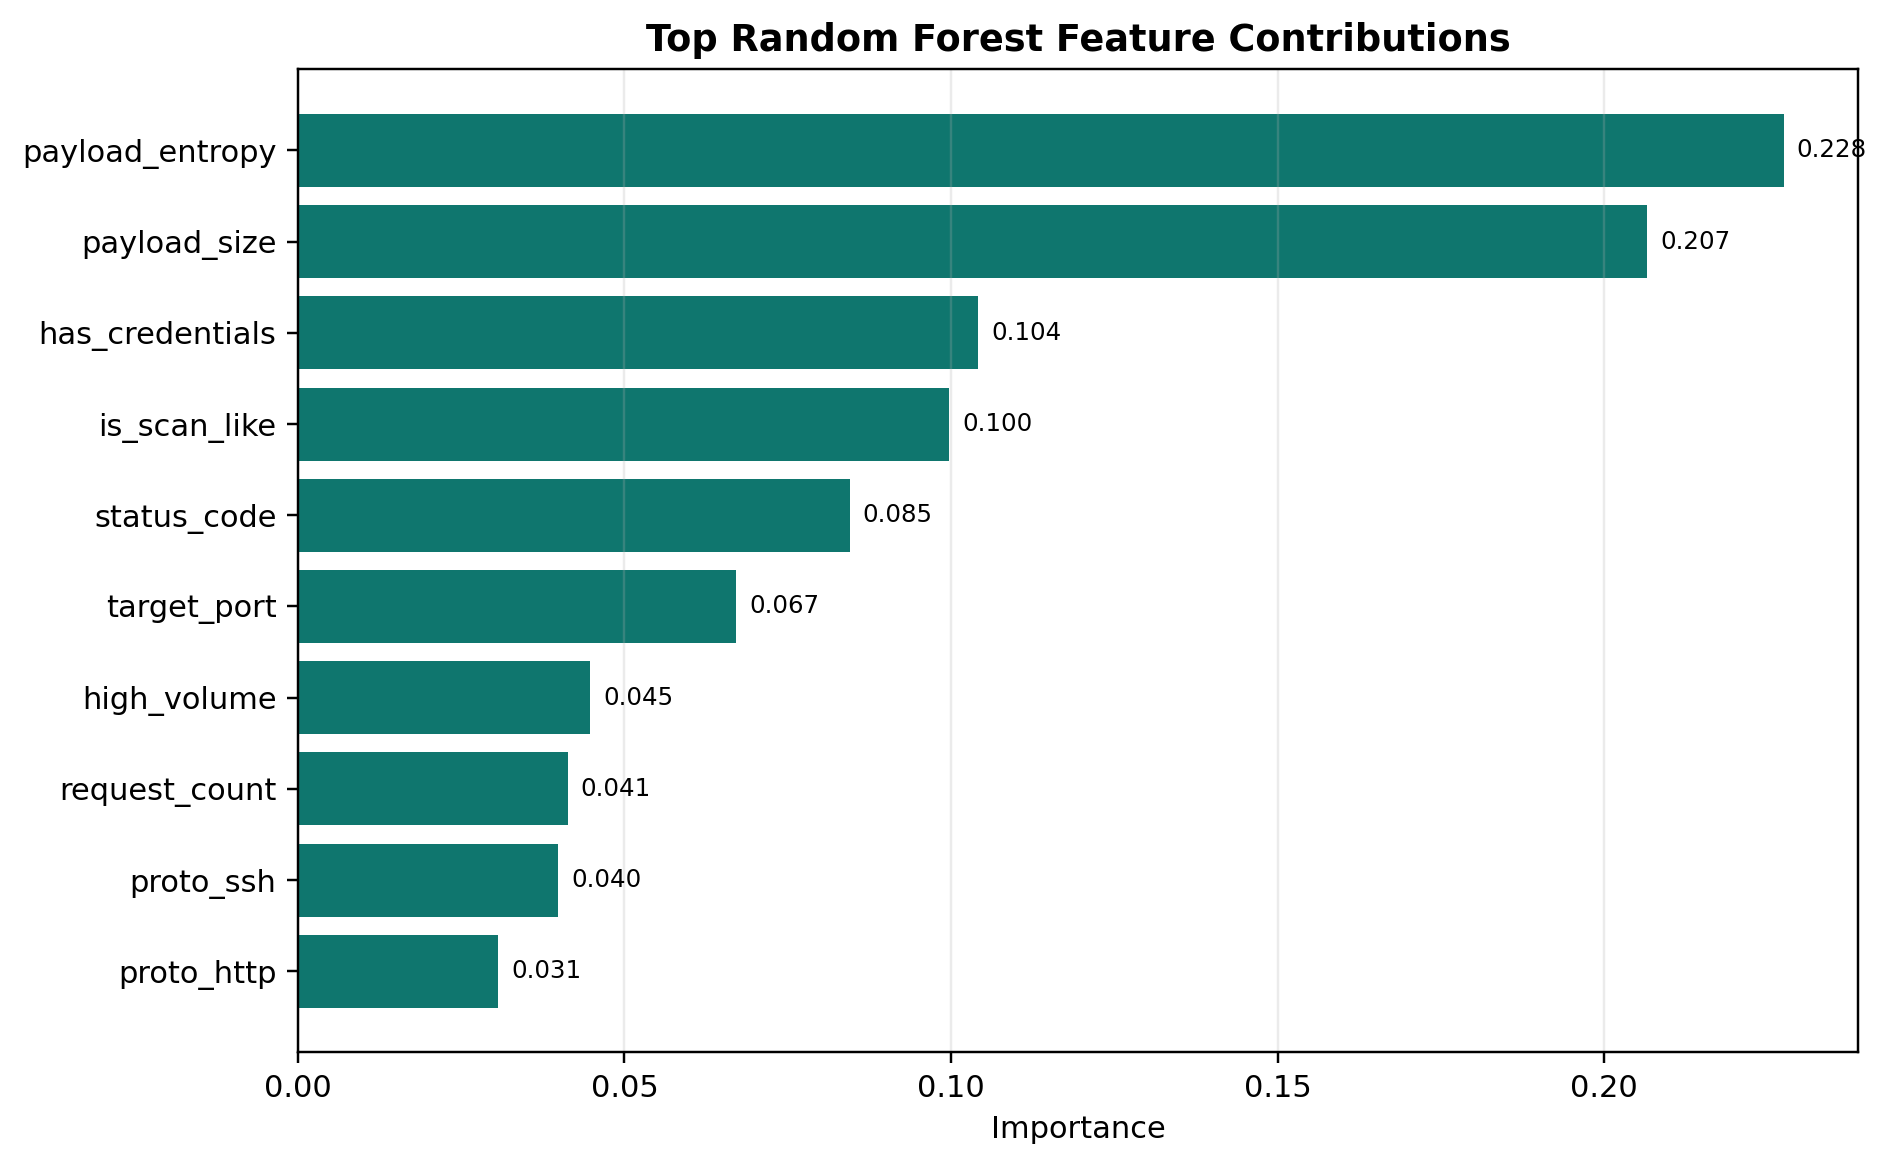
\includegraphics[width=\linewidth]{artifacts/figures/fig07_feature_importance.png}
  \caption{Top feature contributions from the trained Random Forest classifier.}
  \label{fig:importance}
\end{figure}

\subsection{Runtime Dashboard and Evidence Feed}
The running Streamlit dashboard confirmed that the system can ingest and visualize live classified events. Fig. \ref{fig:streamlit-dashboard} shows the threat overview with total events, detected attacks, attacker count, confidence, attack-type distribution, timeline, top attacker IP, and targeted services. The dashboard is intentionally operational: it favors concise counts, trends, and tables over long textual explanations.

\begin{figure}[!t]
  \centering
  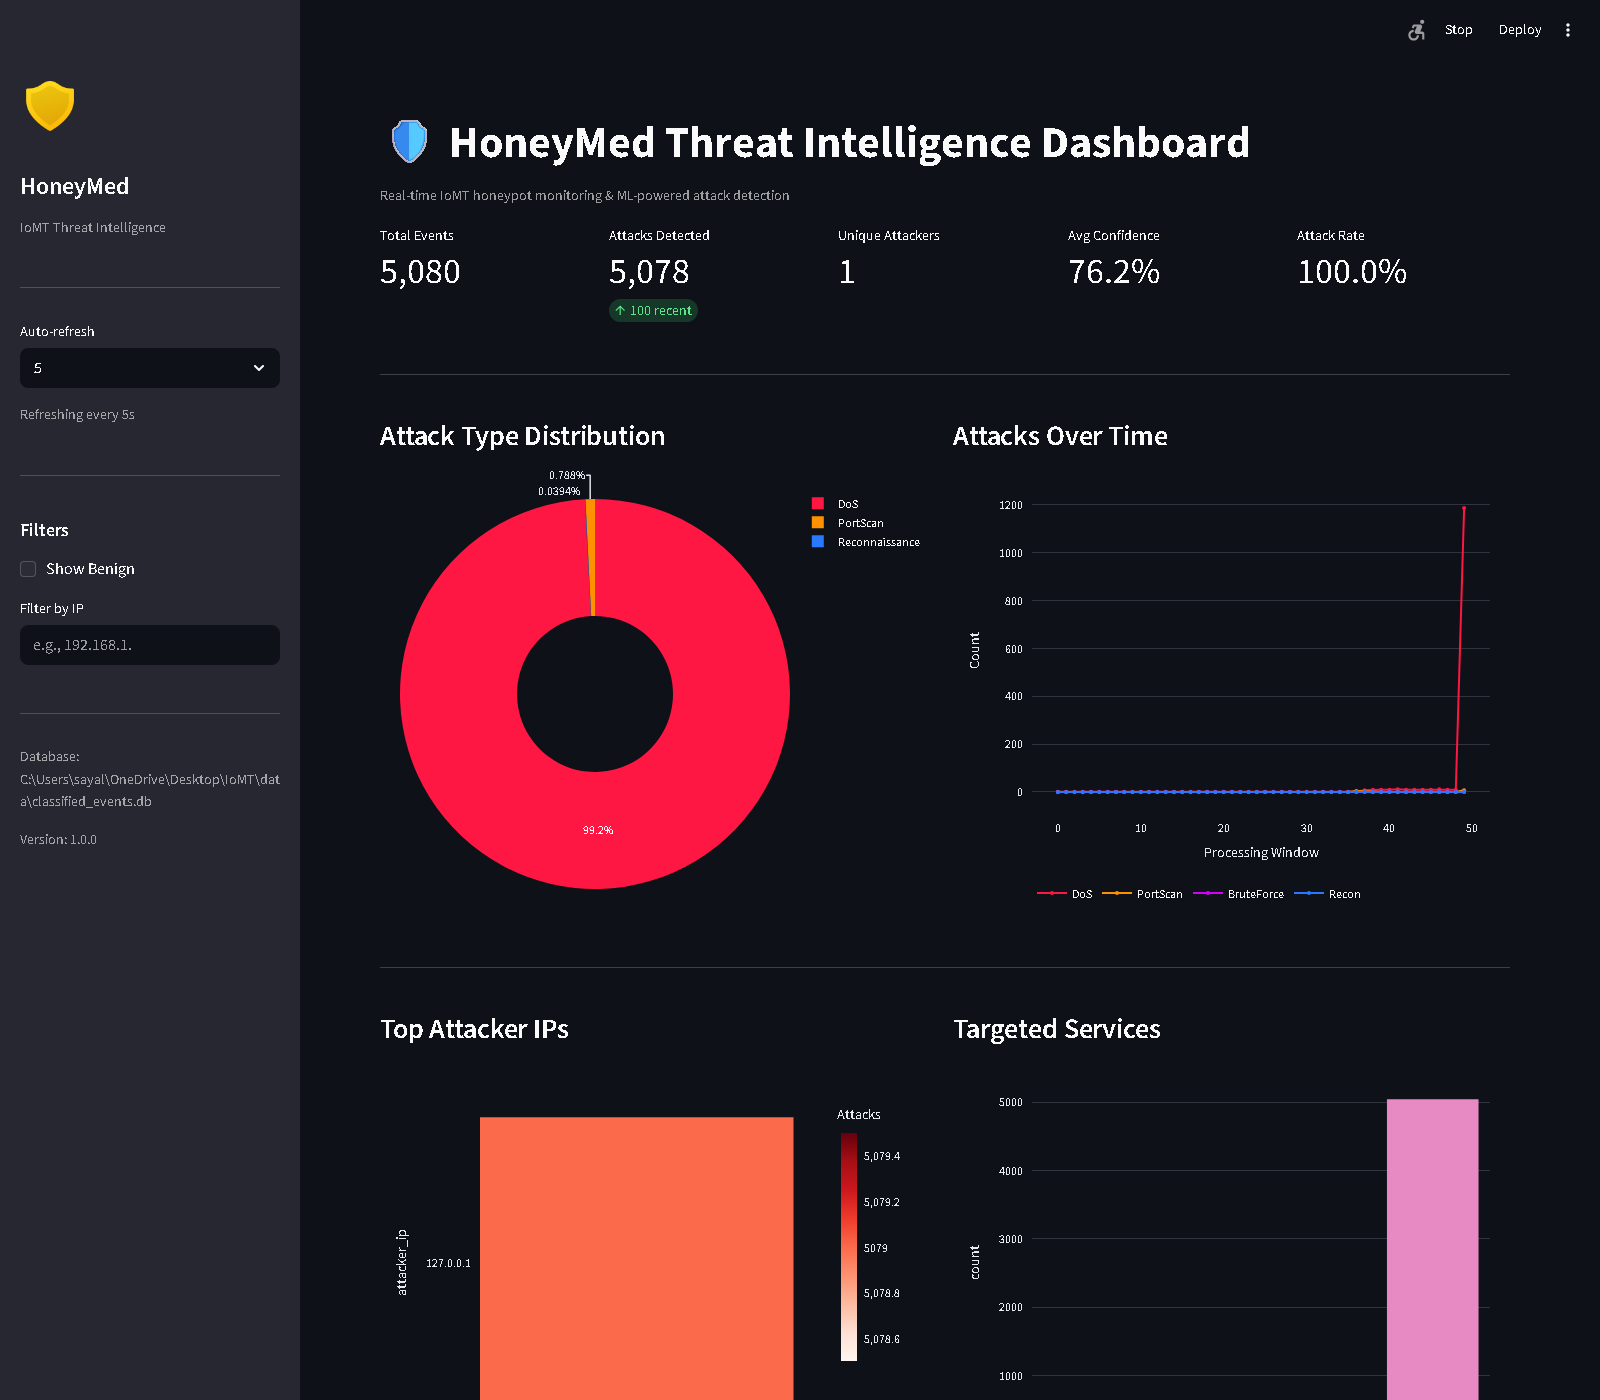
\includegraphics[width=\linewidth]{artifacts/screenshots/fig02_streamlit_threat_dashboard.png}
  \caption{HoneyMed threat dashboard after running the honeypot, real-time pipeline, API, Streamlit app, and attack simulator.}
  \label{fig:streamlit-dashboard}
\end{figure}

Fig. \ref{fig:event-hash-feed} shows the live classified-event feed and hash section. Each event receives a SHA-256 digest, allowing later verification that the stored event record has not changed. In a multi-hospital deployment, this digest can be shared or committed without exposing raw session payloads.

\begin{figure}[!t]
  \centering
  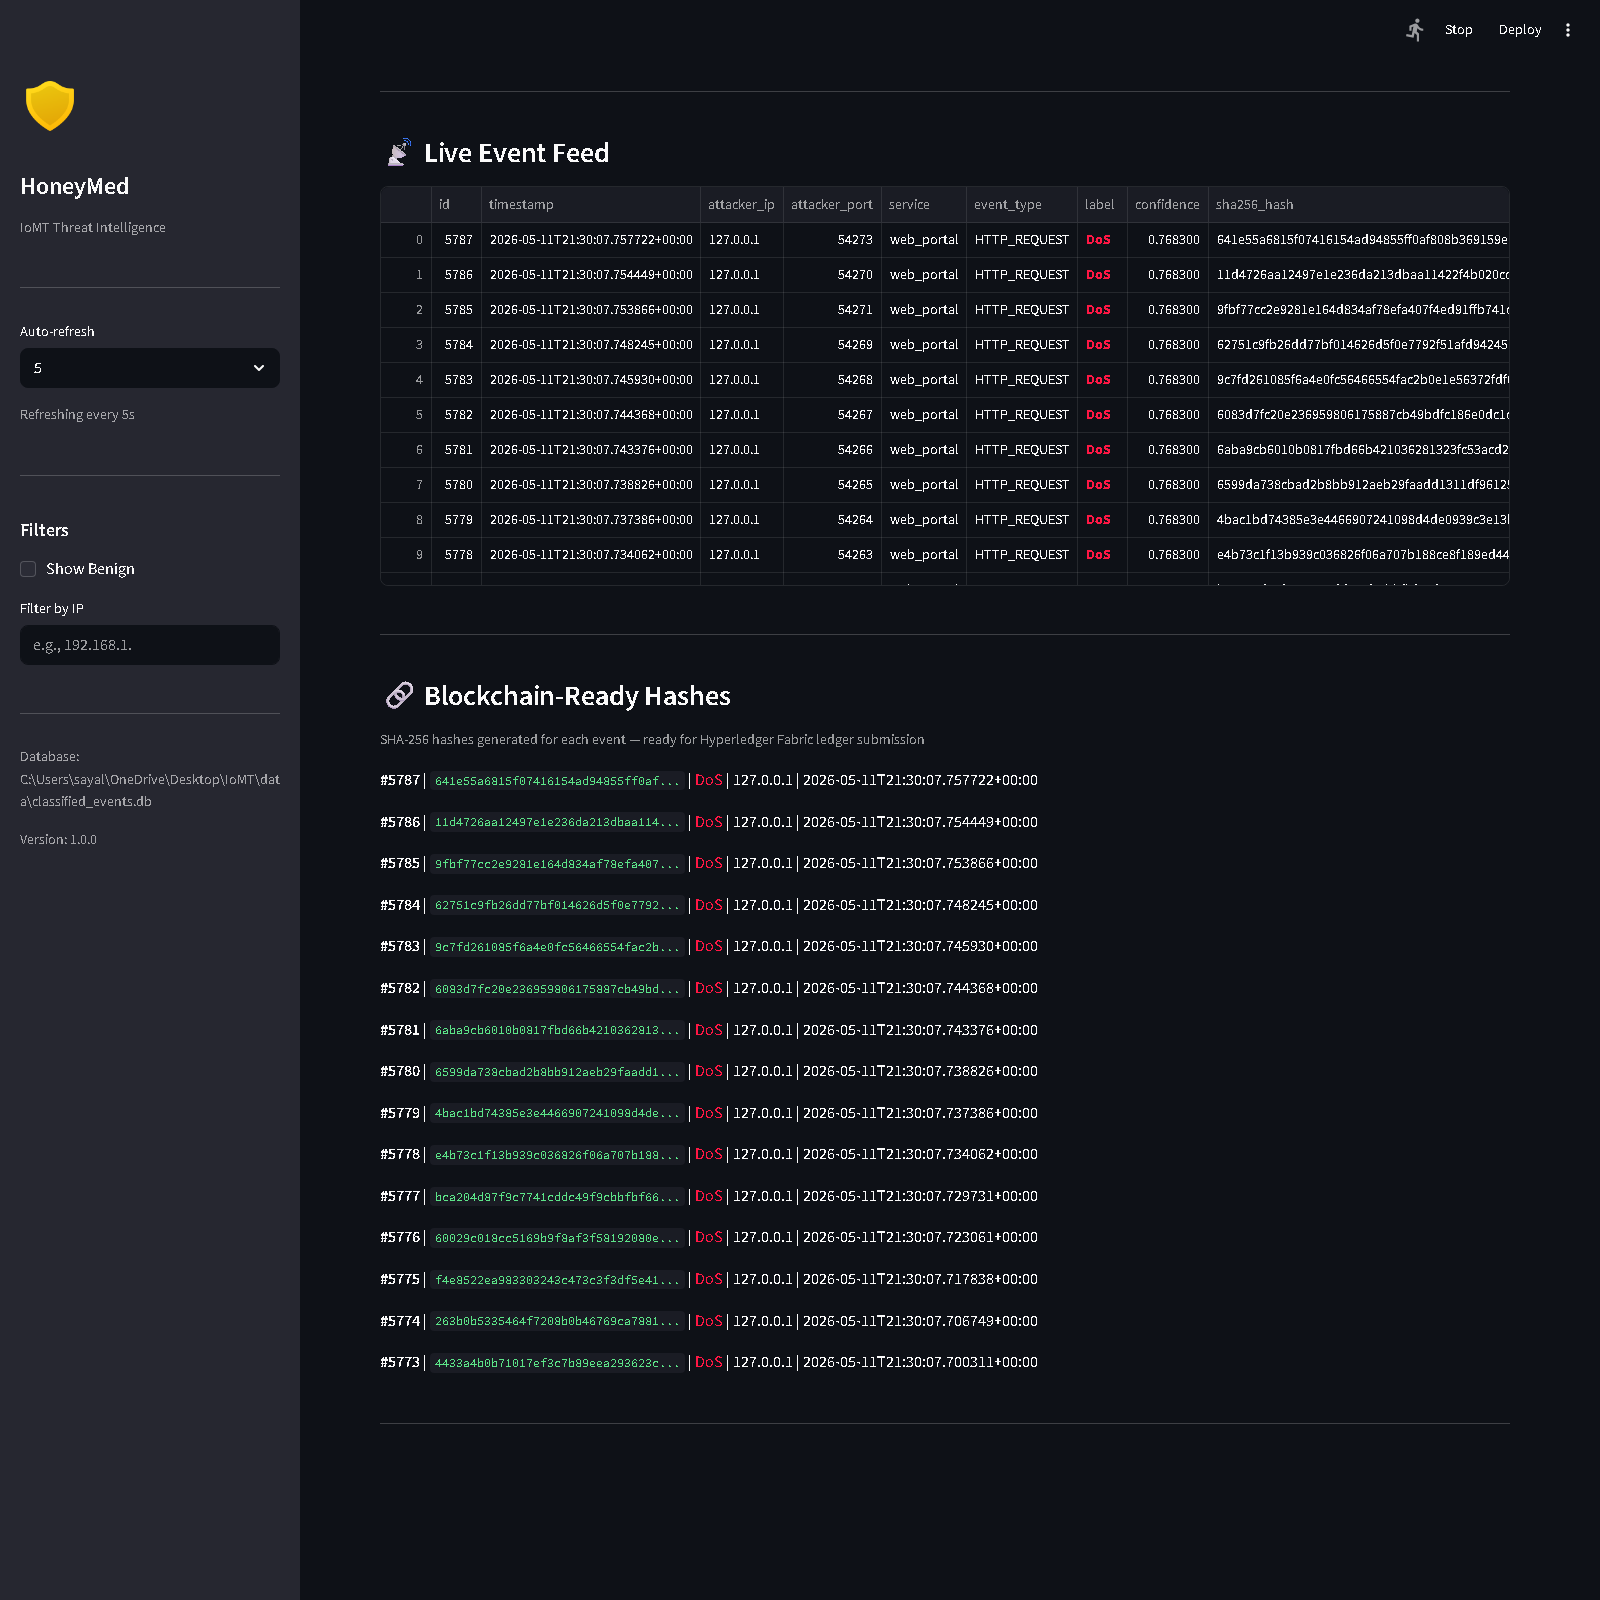
\includegraphics[width=\linewidth]{artifacts/screenshots/fig03_streamlit_events_hashes.png}
  \caption{Live classified-event feed and blockchain-ready SHA-256 hashes generated from processed IoMT honeypot events.}
  \label{fig:event-hash-feed}
\end{figure}

\subsection{Discussion}
The results support three observations. First, a lightweight tree-based model is sufficient for the current prototype. The Random Forest model reached high accuracy with simple engineered features and short training time. Second, the feature-importance plot gives a usable explanation path for analysts. Rather than treating the model as a black box, the system can explain that entropy, payload size, credentials, and scan-like behavior are driving decisions. Third, the dashboard and hash feed demonstrate that the classifier is part of an operational loop, not a standalone notebook result.

There are also limitations. The dataset is generated by the project and the attack traffic is controlled, so the scores should not be read as hospital-production performance. The web flood also dominates the runtime dashboard, which is useful for testing throughput but less balanced than a real deployment. Future work should test the pipeline on CICIoMT2024 and WUSTL-EHMS-2020, add adaptive deception policies, introduce federated model updates, and validate the ledger interface against a real Hyperledger Fabric network.

\section{Conclusion}
HoneyMed demonstrates a practical IoMT honeypot workflow that links medical-protocol deception, real-time feature extraction, supervised attack classification, dashboard visualization, and ledger-ready evidence handling. The latest local experiment trained three classifiers on a 5,000-sample generated dataset and found Random Forest to be the best current model with 98.50\% accuracy and 98.49\% weighted F1-score. Fresh runtime screenshots show that the project runs end to end: the decoy patient monitor is served, attack traffic is captured, classifications are displayed, and SHA-256 hashes are generated for processed events. The main value of HoneyMed is therefore its integration: it turns suspicious IoMT interactions into visible, classified, and auditable security events.

\begin{thebibliography}{00}

\bibitem{lipsa2025interpretable}
S. Lipsa, R. K. Dash, and N. Ivkovic, ``An interpretable dimensional reduction technique with an explainable model for detecting attacks in Internet of Medical Things devices,'' \textit{Scientific Reports}, vol. 15, Art. no. 8718, 2025, doi: 10.1038/s41598-025-93404-8.

\bibitem{hosain2025xaixgboost}
Y. Hosain and M. Cakmak, ``XAI-XGBoost: an innovative explainable intrusion detection approach for securing internet of medical things systems,'' \textit{Scientific Reports}, vol. 15, Art. no. 22278, 2025, doi: 10.1038/s41598-025-07790-0.

\bibitem{ramya2025aidt}
M. Ramya, P. Sudhakaran, Y. Sivagnanam, and C. S. Krishnan, ``Advanced intrusion detection technique (AIDT) for secure communication among devices in internet of medical things (IoMT),'' \textit{EURASIP Journal on Wireless Communications and Networking}, vol. 2025, Art. no. 34, 2025, doi: 10.1186/s13638-025-02462-z.

\bibitem{hassan2025survey}
S. R. Hassan, M. U. Tanveer, S. Prajapat, and M. Shabaz, ``A comprehensive survey on intrusion detection in internet of medical things: Datasets, federated learning, blockchain, and future research directions,'' \textit{ICT Express}, 2025, doi: 10.1016/j.icte.2025.11.005.

\bibitem{abdelhaq2026hybrid}
M. Abdelhaq, S. Palanisamy, M. Gopinath, V. G. S. Manasa, M. A. Ram, and S. Khan, ``A hybrid XGBoost--SVM ensemble framework for robust cyber-attack detection in the internet of medical things (IoMT),'' \textit{Scientific Reports}, vol. 16, Art. no. 6855, 2026, doi: 10.1038/s41598-026-37832-0.

\bibitem{jaiswal2026tsetlin}
R. Jaiswal, P.-A. Andersen, L. R. Cenkeramaddi, L. Jiao, and O.-C. Granmo, ``A Tsetlin Machine-driven intrusion detection system for next-generation IoMT security,'' arXiv:2604.03205, 2026, doi: 10.48550/arXiv.2604.03205.

\bibitem{tawfik2025fedmedsecure}
M. Tawfik, A. A. Abu-Ein, H. M. Noaman, A. H. Abdelhaliem, and I. S. Fathi, ``FedMedSecure: federated few-shot learning with cross-attention mechanisms and explainable AI for collaborative healthcare cybersecurity,'' \textit{Scientific Reports}, vol. 15, Art. no. 40050, 2025, doi: 10.1038/s41598-025-25107-z.

\bibitem{durga2026tinygan}
D. S., M. G. Shankar, E. Daniel, and B. G. V. R., ``Enhancing security in IoMT using federated TinyGAN for lightweight and accurate malware detection,'' \textit{Scientific Reports}, vol. 16, Art. no. 7116, 2026, doi: 10.1038/s41598-026-37830-2.

\bibitem{islam2025fogedge}
U. Islam, M. N. Alatawi, A. Alqazzaz, S. Alamro, B. Shah, and F. Moreira, ``A hybrid fog-edge computing architecture for real-time health monitoring in IoMT systems with optimized latency and threat resilience,'' \textit{Scientific Reports}, vol. 15, Art. no. 25655, 2025, doi: 10.1038/s41598-025-09696-3.

\bibitem{guan2025honeyiot}
C. Guan, J. Zhang, G. Cao, T. F. La Porta, and J. C. Acosta, ``Learning-Based Internet of Things honeypots for cyber deception,'' \textit{IEEE Security \& Privacy}, pp. 2--10, 2025, doi: 10.1109/MSEC.2025.3601986.

\bibitem{li2025deception}
C. Li, N. Zhao, and H. Wu, ``Multiple deception resources deployment strategy based on reinforcement learning for network threat mitigation,'' \textit{Scientific Reports}, vol. 15, Art. no. 16830, 2025, doi: 10.1038/s41598-025-00348-0.

\bibitem{sladic2025vellmes}
M. Sladic, V. Valeros, C. Catania, and S. Garcia, ``VelLMes: A high-interaction AI-based deception framework,'' arXiv:2510.06975, 2025, doi: 10.48550/arXiv.2510.06975.

\bibitem{deb2025taxonomy}
S. Deb, E. Lupu, E. M. Drakakis, A. A. Bharath, Z. K. Leung, G. R. Ma, and A. Chattopadhyay, ``Securing the Internet of Medical Things (IoMT): Real-world attack taxonomy and practical security measures,'' arXiv:2507.19609, 2025, doi: 10.48550/arXiv.2507.19609.

\end{thebibliography}

\end{document}
